\documentclass[14pt,a4paper]{extarticle}
\usepackage{../templates/preamble}

\newcommand{\reportof}{практической работе №2}
\newcommand{\theme}{Полиномы и интерполяция.}

\begin{document}
\begin{titlepage}
    \begin{center}
        {\bfseries
        МИНОБРНАУКИ РОССИИ\par
        САНКТ-ПЕТЕРБУРГСКИЙ ГОСУДАРСТВЕННЫЙ\par
        ЭЛЕКТРОТЕХНИЧЕСКИЙ УНИВЕРСИТЕТ\par
        <<ЛЭТИ>> ИМ. В.И. УЛЬЯНОВА (ЛЕНИНА)\par
        Кафедра \department

        \vspace{0.23\textheight}
        ОТЧЁТ\par
        по \reportof\par
        по дисциплине <<\discipline>>\par
        Тема: \theme
        \vspace{0.28\textheight}
        }
        \begin{table}[!ht]
            \begin{tabularx}{\textwidth}{p{60mm}X>{\centering\arraybackslash}p{45mm}}
                Студент гр. 4352 & \_\_\_\_\_\_\_\_\_\_\_\_\_\_\_\_\_\_\_\_ & {Даричев Е. М.} \\ [5.4mm]  % Line height
                Преподаватель    & \_\_\_\_\_\_\_\_\_\_\_\_\_\_\_\_\_\_\_\_ & {\teacher} \\ [5.4mm]
            \end{tabularx}
        \end{table}

        Санкт-Петербург\par
        \yyear
    \end{center}
\end{titlepage}
\setcounter{page}{2}

% document %
\section*{Цель работы}
    Ознакомиться с методами работы с полиномами и применения
интерполяции.

\section*{Отчёт о проделанной работе}
        В первом задании необходимо подобрать коэффициенты для параболы,
то есть решить задачу интерполяции полиномом второй степени. Запустим код
и попробуем подобрать эти коэффициенты. Проще всего начать с последнего
коэффициента $c$, далее по форме ветвей можно подобрать коэффициент $a$, а
потом и $b$ (рис. \ref{fig:2.1}).

\begin{figure}[h!]
    \centering
    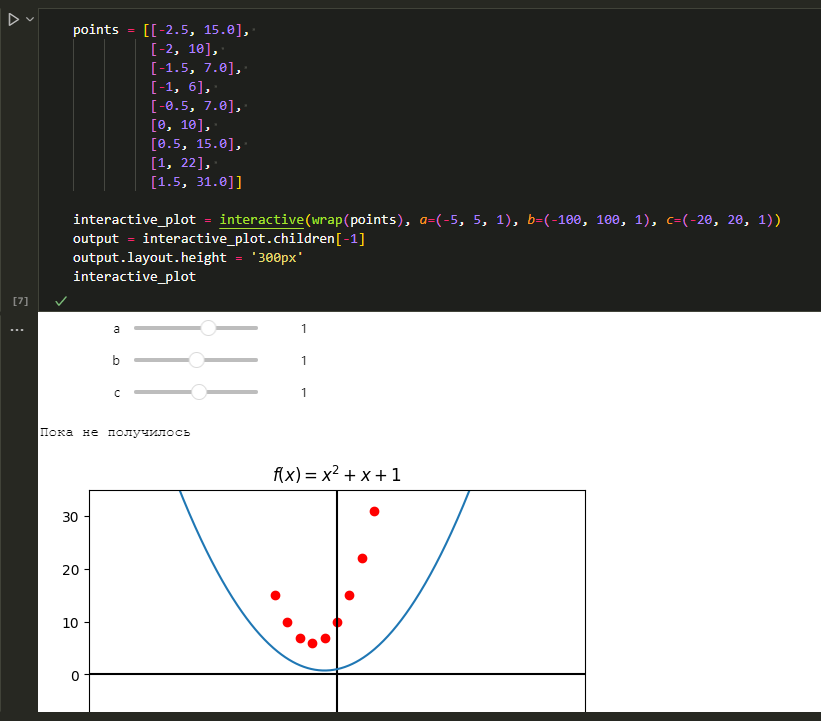
\includegraphics[width=0.4\linewidth]{figures/2.1.png}
    \caption{Программа, создающая ползунки}
    \label{fig:2.1-interactive}
\end{figure}

\begin{figure}[h!]
    \begin{subfigure}{.5\textwidth}
        \centering
        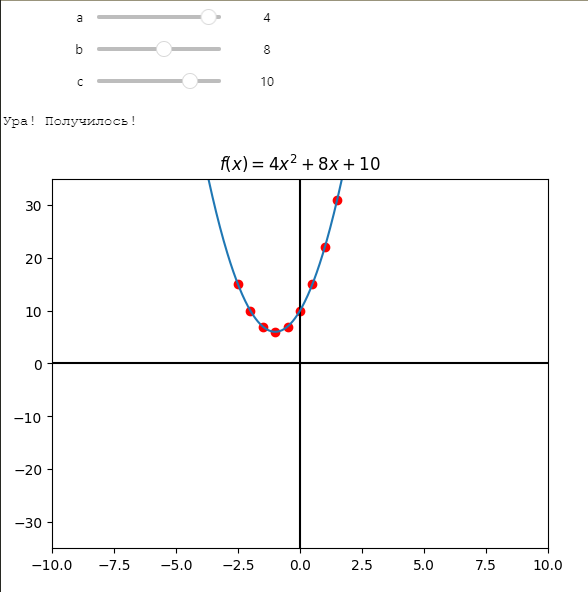
\includegraphics[width=0.9\linewidth]{figures/2.1-first.png}
    \end{subfigure}%
    \begin{subfigure}{.5\textwidth}
        \centering
        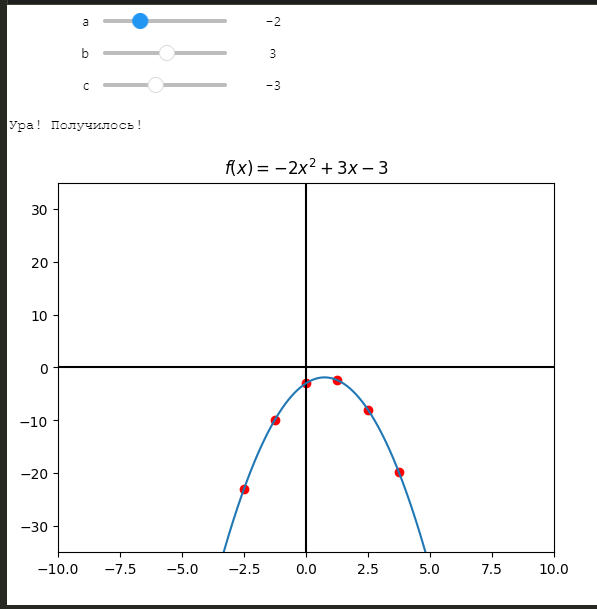
\includegraphics[width=0.9\linewidth]{figures/2.1-second.png}
    \end{subfigure}

    \caption{Задание 2.1}
    \label{fig:2.1}
\end{figure}

        Следующее задание --- найти коэффициенты для кубической параболы,
решить задачу интерполяции полиномом третьей степени. Начнём подбор, как
и в прошлый раз, со свободного коэффициента $a_0$. Далее подберём точку роста
горба с помощью $a_2$ и размер горбов, меняя $a_1$, наконец, прижим параболы
отрегулируем с помощью старшего коэффициента $a_3$ (рис. \ref{fig:2.2}).

\begin{figure}[h!]
    \begin{subfigure}{.5\textwidth}
        \centering
        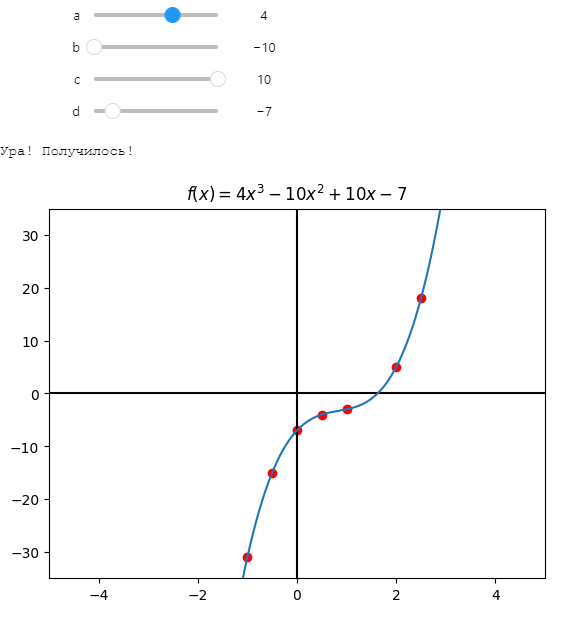
\includegraphics[width=0.9\linewidth]{figures/2.2-first.png}
    \end{subfigure}%
    \begin{subfigure}{.5\textwidth}
        \centering
        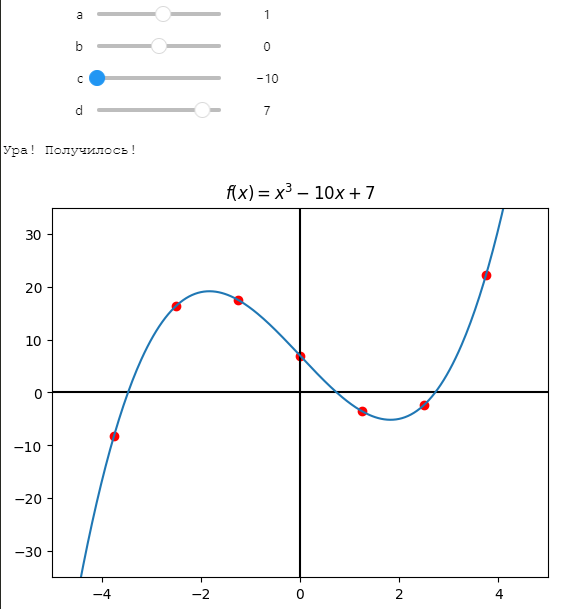
\includegraphics[width=0.9\linewidth]{figures/2.2-second.png}
    \end{subfigure}

    \caption{Задание 2.2}
    \label{fig:2.2}
\end{figure}

        Последнее задание требует аналитического подхода для нахождения
коэффициентов. Для этого напишем код, который будет составлять столько
уравнений, сколько дано точек, а потом решать их (рис \ref{fig:2.3-code}).

\begin{figure}[h!]
    \begin{subfigure}{.5\textwidth}
        \centering
        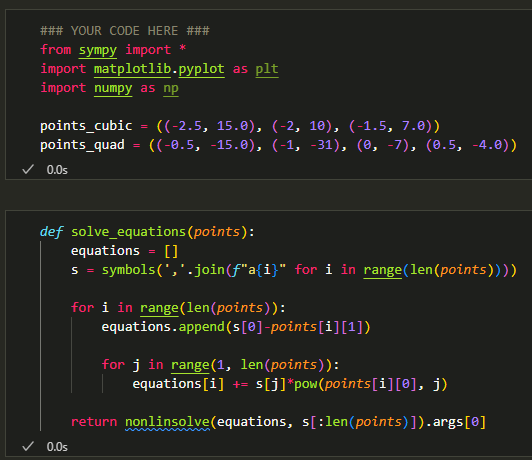
\includegraphics[width=0.9\linewidth]{figures/2.3-code1.png}
    \end{subfigure}%
    \begin{subfigure}{.5\textwidth}
        \centering
        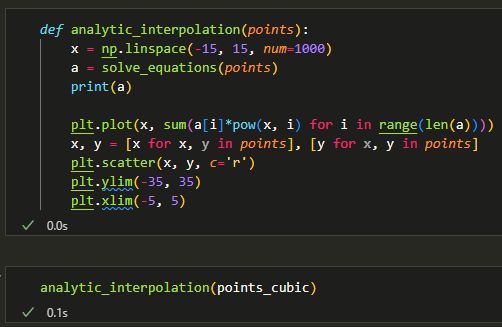
\includegraphics[width=0.9\linewidth]{figures/2.3-code2.png}
    \end{subfigure}

    \caption{Задание 2.3, код программы}
    \label{fig:2.3-code}
\end{figure}

        Ниже на рисунке \ref{fig:2.3-results} приведены результаты работы программы.

\begin{figure}[h!]
    \begin{subfigure}{.5\textwidth}
        \centering
        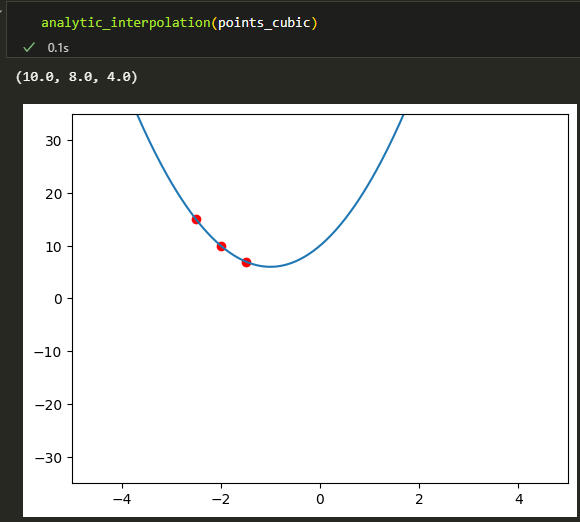
\includegraphics[width=0.9\linewidth]{figures/2.3-res1.png}
    \end{subfigure}%
    \begin{subfigure}{.5\textwidth}
        \centering
        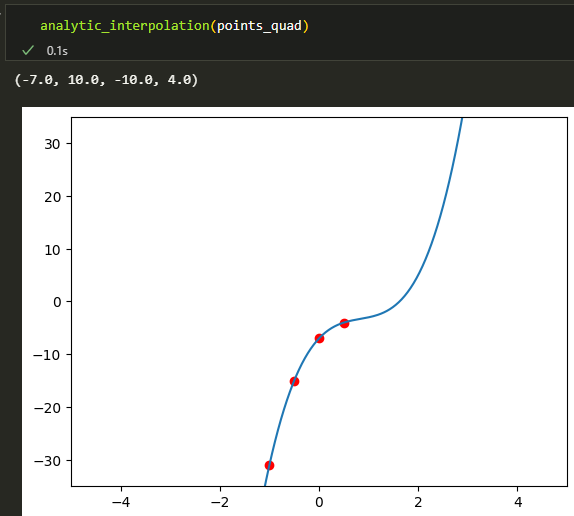
\includegraphics[width=0.9\linewidth]{figures/2.3-res2.png}
    \end{subfigure}

    \caption{Задание 2.3, результаты работы программы}
    \label{fig:2.3-results}
\end{figure}

\section*{Вывод}

        В ходе выполнения работы я узнал о смысле коэффициентов полиномов
второй и третьей степени, научился подбирать эти коэффициенты и строить
графики с помощью библиотеки MatPlotLib.

\end{document}